\documentclass[aspectratio=169,
hyperref={colorlinks,urlcolor=blue}
]{beamer}


%\usetheme{Pittsburgh}
\usetheme{default}
\usepackage{colortbl}%colored tables
%For using helvetica font:
\usepackage[scaled]{helvet}
\usepackage[T1]{fontenc}
\renewcommand\familydefault{\sfdefault}
\urlstyle{same} %sets the fonts for urls
\usepackage{pdfpages}
\usepackage{siunitx}
\usepackage{caption}
\usepackage{pifont}%for dings
\usepackage{pgfplots}%for 3d plotting
\pgfplotsset{compat = newest}
\usepackage{mathtools}%box in align env \Aboxed
\usepackage[american,smartlabels]{circuitikz}%for drawing circuits
\usepackage{multimedia}
\usepackage{animate}
\usepackage{xcolor}


\usetikzlibrary{arrows}
\usetikzlibrary {3d} 
\usetikzlibrary{decorations.markings, math}
\usetikzlibrary{intersections, pgfplots.fillbetween}
\usetikzlibrary {shapes.geometric} 


%\definecolor{myblue}{RGB}{5, 34, 150}
\definecolor{myblue2}{RGB}{5, 34, 150}
\definecolor{myblue}{RGB}{0,36,82}
\definecolor{myred}{RGB}{207, 2, 13}
\definecolor{mygreen}{RGB}{0, 158, 11}
\definecolor{myyellow}{RGB}{220,220,0}
\definecolor{qblue}{RGB}{0,36,82}
\definecolor{qgold}{RGB}{250,189,15}
\definecolor{qred}{RGB}{185,14,49}
\definecolor{cblue}{rgb}{0.13, 0.67, 0.8}
\definecolor{corange}{rgb}{0.8, 0.34, 0.0}
\definecolor{cpurple}{rgb}{0.54, 0.29, 0.42}

%%%%%%%%%%%% General settings
\setbeamercolor{frametitle}{fg=black}
\setbeamercolor{title}{fg=black}
\setbeamercolor{author}{fg=myblue2}

\beamertemplatenavigationsymbolsempty %no navigation controls at bottom of slides
%\setbeamertemplate{footline}[frame number]
\usefonttheme{professionalfonts} 
\setbeamerfont{title}{series=\bfseries,parent=structure}
\setbeamerfont{frametitle}{series=\bfseries,parent=structure}

%%%%%%%%%%%%Lists
\setbeamertemplate{itemize item}[circle] %{\color{myblue}$\circ$}
\setbeamertemplate{itemize subitem}{\color{myblue2}$\circ$}
\setbeamertemplate{itemize subsubitem}{\color{myblue2}$\cdot$}
\setbeamercolor{itemize item}{bg=myblue2,fg=myblue2}
\setbeamercolor{enumerate item}{bg=myblue2,fg=myblue2}
%%%%%%%%%%%%%%%%%%%%%%%%%%%%

%%%%%%%%%%%%Blocks
\setbeamertemplate{blocks}[rounded]
%Default block
\setbeamercolor{block title}{bg=myblue2, fg=white}
\setbeamercolor{block body}{bg=myblue2!10}
\setbeamerfont{block body}{size=\scriptsize}
\setbeamerfont{block title}{size=\scriptsize}
%Alert block
\setbeamercolor{block title alerted}{bg= myblue2, fg=white}
\setbeamercolor{block body alerted}{bg=myblue2!10}
\setbeamerfont{block body alerted}{size=\scriptsize}
\setbeamerfont{block title alerted}{size=\scriptsize}
%example block
\setbeamercolor{block title example}{bg=mygreen, fg=white}
\setbeamercolor{block body example}{bg=mygreen!10}
\setbeamerfont{block body example}{size=\scriptsize}
\setbeamerfont{block title example}{size=\scriptsize}
%%%%%%%%%%%%%%%%55


%%%%%%%%%%%%Figures and captions
\captionsetup{font=scriptsize,labelfont=scriptsize}
%\setbeamertemplate{caption}{\raggedright\insertcaption\par}
\newenvironment{capfig}[3]{\begin{figure}\includegraphics[width=#1\textwidth]{#2}\caption*{\textit{#3}}\end{figure}}{}

%\makeatother
%\setbeamertemplate{footline}
%{
%  \leavevmode%
%  \hbox{%
%  \begin{beamercolorbox}[wd=.4\paperwidth,ht=2.25ex,dp=1ex,center]{author in head/foot}%
%    \usebeamerfont{author in head/foot}\insertshortauthor
%  \end{beamercolorbox}%
%  \begin{beamercolorbox}[wd=.6\paperwidth,ht=2.25ex,dp=1ex,center]{title in head/foot}%
%    \usebeamerfont{title in head/foot}\insertshorttitle\hspace*{3em}
%    \insertframenumber{} / \inserttotalframenumber\hspace*{1ex}
%  \end{beamercolorbox}
%  }%
%  \vskip0pt%
%}
%\makeatletter

\makeatother
\setbeamertemplate{footline}
{
  \leavevmode%
  \hbox{%
\begin{beamercolorbox}[wd=.27\paperwidth,ht=2.25ex,dp=1ex,center]{author in head/foot}%
    \color{black}{\insertinstitute}
\end{beamercolorbox}
  \begin{beamercolorbox}[wd=.27\paperwidth,ht=2.25ex,dp=1ex,center]{author in head/foot}%
    \color{black}{\inserttitle}
  \end{beamercolorbox}%
  \begin{beamercolorbox}[wd=.27\paperwidth,ht=2.25ex,dp=1ex,center]{title in head/foot}%
    \color{black}{\insertshortauthor}
  \end{beamercolorbox}
  \begin{beamercolorbox}[wd=.27\paperwidth,ht=2.25ex,dp=1ex,center]{title in head/foot}%
    \hspace{.28\paperwidth}\color{black} \insertframenumber{} / \inserttotalframenumber\hspace*{1ex}
  \end{beamercolorbox}
  }%
  \vskip0pt%
}
\makeatletter

\setbeamertemplate{title page}
{
  \begin{tikzpicture}[remember picture,overlay]
    \def\barh{4}%15
  
    \draw[color=myblue2,line width=\barh] ([yshift=-0.5*\barh]current page.north west) -- ([yshift=-0.5*\barh,xshift=-0.67\paperwidth]current page.north east);
    \draw[color=myblue2,line width=\barh] ([yshift=-0.5*\barh,xshift=-0.67\paperwidth]current page.north east) -- ([yshift=-0.5*\barh,xshift=-0.34\paperwidth]current page.north east);
    \draw[color=myblue2,line width=\barh] ([yshift=-0.5*\barh,xshift=-0.34\paperwidth]current page.north east) -- ([yshift=-0.5*\barh]current page.north east); 
  
    \draw[color=myblue2,line width=\barh] ([yshift=0.5*\barh]current page.south west) -- ([yshift=0.5*\barh,xshift=-0.67\paperwidth]current page.south east);
    \draw[color=myblue2,line width=\barh] ([yshift=0.5*\barh,xshift=-0.67\paperwidth]current page.south east) -- ([yshift=0.5*\barh,xshift=-0.34\paperwidth]current page.south east);
    \draw[color=myblue2,line width=\barh] ([yshift=0.5*\barh,xshift=-0.34\paperwidth]current page.south east) -- ([yshift=0.5*\barh]current page.south east);
    %\node[left] at (current page.east) {
    %
\includegraphics[scale=0.1]{figures/coverpage}
    %};
  \end{tikzpicture}
  
  \usebeamerfont{title}\usebeamercolor[fg]{title}\inserttitle\par
  \usebeamerfont{subtitle}\usebeamercolor[fg]{subtitle}\insertsubtitle\par
  \vspace{2cm}
  \usebeamerfont{author}\usebeamercolor[fg]{author}\insertauthor\par
  \usebeamerfont{institute}\usebeamercolor[fg]{author}\insertinstitute\par
  \usebeamercolor[fg]{author}\par
  \usebeamercolor[fg]{titlegraphic}\inserttitlegraphic

} 

\setbeamertemplate{frametitle}{%
    \nointerlineskip%
        \par\hspace*{-\dimexpr0.5\paperwidth-0.5\textwidth}\textcolor{myblue2}{\rule{0.33\paperwidth}{6pt}}\textcolor{myblue2}{\rule{0.33\paperwidth}{6pt}}\textcolor{myblue2}{\rule{0.34\paperwidth}{6pt}} 
    \begin{beamercolorbox}[wd=\paperwidth,ht=0.75cm,dp=0.6ex]{frametitle}
        \hspace*{0.5cm}\strut\usebeamerfont{frametitle}\insertframetitle\strut
        %\hrule
    \end{beamercolorbox}%
    %%Line below:
%\par\hspace*{-\dimexpr0.5\paperwidth-0.5\textwidth}\textcolor{myblue}{\rule{\paperwidth}{0.4pt}}
     % <-- calculation of left margin width + rule
     %\textcolor{red}{\noindent\rule{\paperwidth}{2pt}}
}


%%%%%%%%%%%%Frame templates

%Slide with title
\newenvironment{titleframe}[1]
{\begin{frame}\frametitle{#1}\end{frame}}
{}

%Slide with title and itemize list:
\newenvironment{bulletframe}[1]
{\begin{frame}{#1} \itemize}
{\enditemize \end{frame}}

%Slide with two columns 50/50
\newenvironment{twocolframe}[3]
{\begin{frame}{#1}
 \begin{columns}[T]
 \column{0.5\textwidth}#2
 \column{0.5\textwidth}#3
 \end{columns}\end{frame}}{}

%Slide with two columns 60/40 <<<<<<<<<<<<<<<<<<<<<<  This one!
\newenvironment{twocolframesf}[3]
{\begin{frame}{#1}
 \begin{columns}[T]
 \column{0.6\textwidth}#2
 \column{0.4\textwidth}#3
 \end{columns}\end{frame}}{}
 
%Slide with two columns 70/30
\newenvironment{twocolframest}[3]
{\begin{frame}{#1}
 \begin{columns}[T] 
 \column{0.7\textwidth}#2
 \column{0.3\textwidth}#3
 \end{columns}\end{frame}}{} 
 
%Slide with two columns 40/60
\newenvironment{twocolframefs}[3]
{\begin{frame}{#1}
 \begin{columns}[T] 
 \column{0.4\textwidth}#2
 \column{0.6\textwidth}#3
 \end{columns}\end{frame}}{}
 
%Slide with two columns 70/30
\newenvironment{twocolframets}[3]
{\begin{frame}{#1}
 \begin{columns}[T] 
 \column{0.3\textwidth}#2
 \column{0.7\textwidth}#3
 \end{columns}\end{frame}}{} 

 
%Colloquium speaker (title, abstract, picture file, speaker name)
\newenvironment{colloquium}[5]
{
\begin{frame}{Colloquium: Friday 1:30pm in Stirling A}
\begin{columns}[T] 
 \column{0.8\textwidth}
 \textbf{#1}\\
 #2
 \column{0.2\textwidth}
 \capfig{#3}{#4}{#5}
 \end{columns}
\end{frame}
}
{} 

%%%%%%%%%%%%%Set Hyperref colors


\hypersetup{
  colorlinks=true,
  linkcolor=blue,    
  urlcolor=blue,     
  citecolor=blue      
}
%%%%%%%%%%%%%TOC bolding
\setbeamerfont{section in toc}{series=\bfseries}


\setcounter{tocdepth}{3}
%Frames:
% \twocolframesf 60/40 (fs, st, ts) 
% \titleframe
% bulletframe


%%%%%%%%%%%%%%%%%%%%%%%%%
%%%%%% START OF PRESENTATION %%%%%%
%%%%%%%%%%%%%%%%%%%%%%%%%

\title{Applying Newton's Laws}
\subject{Motion, Derivations and Modelling Situations}
\subtitle{Building Models to Describe our World}


\begin{document}

%%%%%%%%%%%%%%%%%%%%%%%%%
%%%%%% Title slide %%%%%%
%%%%%%%%%%%%%%%%%%%%%%%%%
\chaptertitle{Applying Newton's Laws}
\begin{frame}
\titlepage
\thispagestyle{empty}

\begin{textblock*}{5cm}(11cm,4cm)
    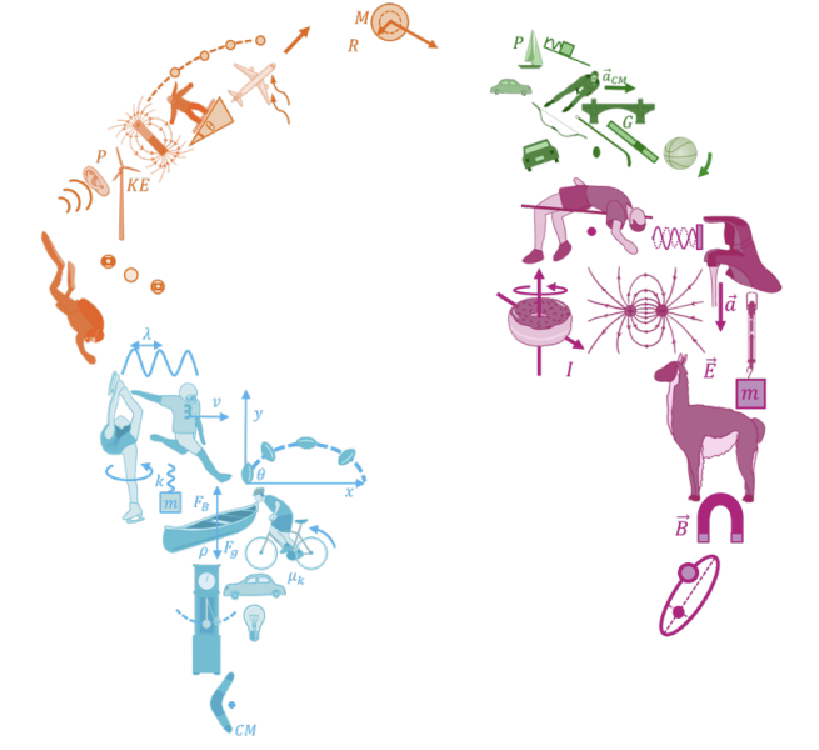
\includegraphics[width=4cm]{figures/BMDW/logo}
\end{textblock*}

\end{frame}
%%%%%%%%%%%%%%%%%%%%%%%%


\twocolframe{Outline}
{\tableofcontents[sections=1, subsectionstyle=show/show]\thispagestyle{empty}}
{\tableofcontents[sections=2-3, subsectionstyle=show/show]}







%%%%%%%%%%%%%%%%%%%%%%%%%%%%%%%%
\section{Types of Motion}
\label{sec:typesofmotion}
\title{Types of Motion}


%%%%%%%%%%%%%%%%%%%%%%%%%
\begin{frame}
\titlepage
\thispagestyle{empty}
\end{frame}



%%%%%%%%%%%%%%%%%%%%%%%
\subsection{Linear motion}
\label{subsec:linearmotion}
\begin{frame}{Linear motion}
\begin{itemize}
\item We can loosely define ``linear motion'' as motion along a straight line, where the velocity does not change direction.
\item The net force (and acceleration) is co-linear with the velocity.
\item We can break up many types of motion into segments where the motion is linear along the segments.
\end{itemize}

\begin{center}
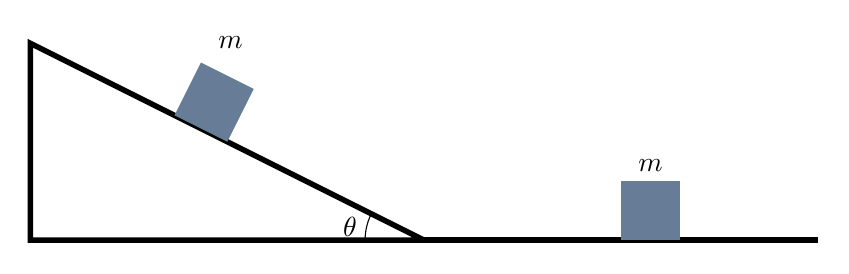
\begin{tikzpicture}[scale=1]
\tikzmath{
\L=5;
\h=2.5;
\abox=0.75;
\R=0.5*\abox;
\th=atan(\h/\L);
\d=\R+\L*cos(\th)/2;
}
\scalebox{1.0}{
\coordinate (Pb1) at (\L/2,\h/2);%coordinates of box
\coordinate (Pb2) at ($(Pb1)+(180-\th:\abox)$);
\coordinate (Pb3) at ($(Pb2)+(90-\th:\abox)$);
\coordinate (Pb4) at ($(Pb3)+(-\th:\abox)$);

%plane and angle
\draw[line width=2pt] (0,\h) -- (0,0) -- (\L,0) -- cycle;
\draw[line width=2pt] (\L,0) -- (2*\L,0);
\draw (\L-0.75,0) arc(180:180-\th:0.75) node[midway,left]{$\theta$};


%boxes
\fill[color=myblue!60] (Pb1) -- (Pb2) -- (Pb3) -- (Pb4) -- cycle ;
\fill[color=myblue!60] (1.5*\L,0) rectangle (1.5*\L+\abox,\abox);

\node at ($(Pb3)+(\abox/2,\abox/3)$) {$m$};
\node[above] at (1.5*\L+0.5*\abox,\abox) {$m$};
}
\end{tikzpicture}
\captionof*{figure}{\textit{A block slides down an incline and then a flat section. Both segments are linear motion.}}
\end{center}

\end{frame}


%%%%%%%%%%%%%%%%%%%%%%%%%%%%%%%%
\subsection{Constant net force}
\label{subsec:cnstnetforce}
\begin{frame}{Constant net force}
\begin{itemize}
\item When the \textbf{sum of the forces} (aka the net force) on an object is constant (in magnitude and direction), and the mass of the object is constant, the acceleration of that object is constant:
\begin{align*}
\sum \vec F = \vec F^{net}=m\vec a
\end{align*}
\item When the acceleration is constant:
\begin{align*}
\vec v(t) &= \vec v_0+\vec at=\vec v_0+\frac{\vec F^{net}}{m}t\\
\vec r(t) &= \vec r_0+\vec v_0 t+\frac{1}{2}\vec a t^2=\vec r_0+\vec v_0 t+\frac{1}{2} \frac{\vec F^{net}}{m} t^2
\end{align*}
\item This is a vector equation, so true by component, for example, the $x$ component:
\begin{align*}
v_x(t)=v_{0x}+\frac{F_x}{m}t\quad x(t)=x_0+v_{0x}t+\frac{1}{2}\frac{F_x}{m}t^2
\end{align*}
\end{itemize}

\end{frame}


%%%%%%%%%%%%%%%%%%%%%%%%%%%%%%%%
\subsection{Varying net force}
\label{subsec:varying net force}
\begin{frame}{Varying net force}
\begin{itemize}
\item The net force on an object can change magnitude and direction:
\begin{itemize}
\item As a function of time.
\item As a function of position.
\item As a function of velocity.
\end{itemize}
\item Then, the acceleration is not constant, and we have to start with:
\begin{align*}
\frac{d\vec v}{dt}&=\vec a = \frac{\vec F^{net}}{m}\\
\frac{d\vec r}{dt}&=\vec v
\end{align*}
and integrate...
\end{itemize}

\end{frame}


%%%%%%%%%%%%%%%%%%%%%%%%%%%%%%%%
\subsubsection{Varying with time}
\label{subsubsec:varyingwithtime}
\begin{frame}{Linear motion, force varies with time}
\begin{itemize}
\item If the magnitude of the force changes with time:
\begin{align*}
\vec a(t)=\frac{\vec F^{net}(t)}{m}
\end{align*}
\item The kinematics equations are ``straightforward'':
\begin{align*}
\frac{d\vec v}{dt}&=\frac{1}{m}\vec F^{net}(t)\\
\therefore \vec v(t)&=\vec v_0+\frac{1}{m}\int_0^t \vec F^{net}(t) dt\\
\therefore \vec r(t)&=\vec r_0+\int_0^t \vec v(t) dt\\
\end{align*}
just some integrals that you can look up if you know the function $\vec F^{net}(t)$...
\end{itemize}

\end{frame}


%%%%%%%%%%%%%%%%%%%%%%%%%%%%%%%%


%%%%%%%%%%%%%%%%%%%%%%%%%%%%%%%%
\subsubsection{Varying with position}
\label{subsubsec:varyingwithposition}
\begin{frame}{Linear motion, force varies with position}
\begin{itemize}
\item If the magnitude of the force changes with position of the object:
\begin{align*}
 a_x(x)=\frac{F^{net}_x(x)}{m}
\end{align*}
\item We cannot ``simply integrate'' the equations that define acceleration from velocity and velocity from position:
\begin{align*}
\frac{dv_x}{dt}=a_x(x) \rightarrow v_x(t)=v_{0x}+\int_0^ta_x(x)dt
\end{align*}
\end{itemize}

\only<2>{
\begin{tikzpicture}[remember picture,overlay]
\coordinate (X1) at ($(current page.center)+(-0.5,0.35)$);
\coordinate (X2) at ($(X1)+(0,-1)$);
\coordinate (X3) at ($(X1)+(4.5,0)$);
\coordinate (X4) at ($(X3)+(0,-1)$);

\draw[color=myred,line width=5] (X1) -- (X4);
\draw[color=myred,line width=5] (X3) -- (X2);

\end{tikzpicture}
}

\begin{center}
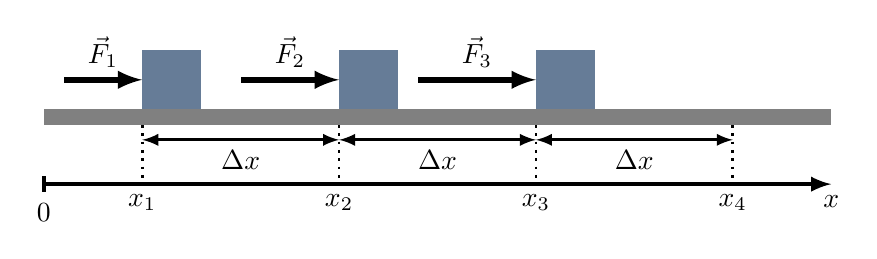
\begin{tikzpicture}[scale=1]
\tikzmath{
\L=10;
\h=0.75;
\w=0.2;
\dx=2.5;
\abox=0.75;
\Fm=1;
}
\scalebox{1.0}{
%axis
\draw[-latex, line width=1.5pt] (0,0) -- (\L,0) node[below]{$x$};
\draw[line width=1.5pt] (0,0.1) -- (0,-0.1) node[below]{$0$};
%floor
\fill[black!50] (0,\h) rectangle (\L,\h+\w);

\fill[color=myblue!60] (0.5*\dx,\h+\w) rectangle (0.5*\dx+\abox,\h+\w+\abox);
\fill[color=myblue!60] (1.5*\dx,\h+\w) rectangle (1.5*\dx+\abox,\h+\w+\abox);
\fill[color=myblue!60] (2.5*\dx,\h+\w) rectangle (2.5*\dx+\abox,\h+\w+\abox);

\draw[latex-,line width=2] (0.5*\dx,\h+\w+\abox/2) -- +(-\Fm,0) node[midway,above]{$\vec F_1$};
\draw[latex-,line width=2] (1.5*\dx,\h+\w+\abox/2) -- +(-1.25*\Fm,0) node[midway,above]{$\vec F_2$};
\draw[latex-,line width=2] (2.5*\dx,\h+\w+\abox/2) -- +(-1.5*\Fm,0) node[midway,above]{$\vec F_3$};

\draw[dotted, line width=1] (0.5*\dx,\h) -- +(0,-\h) node[below]{$x_1$};
\draw[dotted, line width=1] (1.5*\dx,\h) -- +(0,-\h) node[below]{$x_2$};
\draw[dotted, line width=1] (2.5*\dx,\h) -- +(0,-\h) node[below]{$x_3$};
\draw[dotted, line width=1] (3.5*\dx,\h) -- +(0,-\h) node[below]{$x_4$};

\draw[latex-latex, line width=1] (0.5*\dx,0.75*\h)--+(\dx,0) node[midway, below]{$\Delta x$};
\draw[latex-latex, line width=1] (1.5*\dx,0.75*\h)--+(\dx,0) node[midway, below]{$\Delta x$};
\draw[latex-latex, line width=1] (2.5*\dx,0.75*\h)--+(\dx,0) node[midway, below]{$\Delta x$};
}
\end{tikzpicture}
\captionof*{figure}{\textit{A block slides along $x$ with a force that changes depending on position.}}
\end{center}
\end{frame}



%%%%%%%%%%%%%%%%%%%%%%%%%%%%%%%%
\subsection{Breaking up motion}
\label{subsec:breakingupmotion}
\begin{frame}{Breaking it up}
\begin{itemize}
\item When things vary continuously, we can break up the motion into small segments where things are constant (in this case, things = force, acceleration).
\end{itemize}

\begin{center}
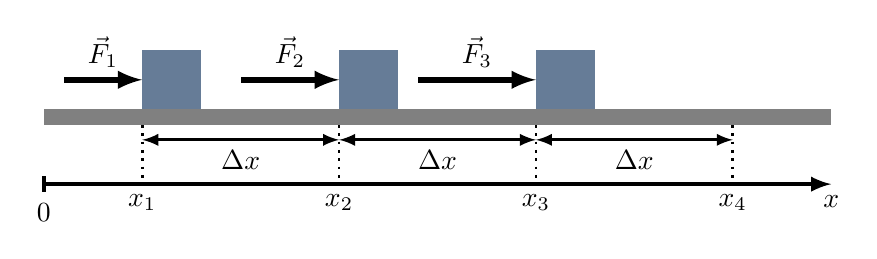
\begin{tikzpicture}[scale=1]
\tikzmath{
\L=10;
\h=0.75;
\w=0.2;
\dx=2.5;
\abox=0.75;
\Fm=1;
}
\scalebox{1.0}{
%axis
\draw[-latex, line width=1.5pt] (0,0) -- (\L,0) node[below]{$x$};
\draw[line width=1.5pt] (0,0.1) -- (0,-0.1) node[below]{$0$};
%floor
\fill[black!50] (0,\h) rectangle (\L,\h+\w);

\fill[color=myblue!60] (0.5*\dx,\h+\w) rectangle (0.5*\dx+\abox,\h+\w+\abox);
\fill[color=myblue!60] (1.5*\dx,\h+\w) rectangle (1.5*\dx+\abox,\h+\w+\abox);
\fill[color=myblue!60] (2.5*\dx,\h+\w) rectangle (2.5*\dx+\abox,\h+\w+\abox);

\draw[latex-,line width=2] (0.5*\dx,\h+\w+\abox/2) -- +(-\Fm,0) node[midway,above]{$\vec F_1$};
\draw[latex-,line width=2] (1.5*\dx,\h+\w+\abox/2) -- +(-1.25*\Fm,0) node[midway,above]{$\vec F_2$};
\draw[latex-,line width=2] (2.5*\dx,\h+\w+\abox/2) -- +(-1.5*\Fm,0) node[midway,above]{$\vec F_3$};

\draw[dotted, line width=1] (0.5*\dx,\h) -- +(0,-\h) node[below]{$x_1$};
\draw[dotted, line width=1] (1.5*\dx,\h) -- +(0,-\h) node[below]{$x_2$};
\draw[dotted, line width=1] (2.5*\dx,\h) -- +(0,-\h) node[below]{$x_3$};
\draw[dotted, line width=1] (3.5*\dx,\h) -- +(0,-\h) node[below]{$x_4$};

\draw[latex-latex, line width=1] (0.5*\dx,0.75*\h)--+(\dx,0) node[midway, below]{$\Delta x$};
\draw[latex-latex, line width=1] (1.5*\dx,0.75*\h)--+(\dx,0) node[midway, below]{$\Delta x$};
\draw[latex-latex, line width=1] (2.5*\dx,0.75*\h)--+(\dx,0) node[midway, below]{$\Delta x$};
}
\end{tikzpicture}
\captionof*{figure}{\textit{A block slides along $x$ with a force that changes depending on position.}}
\end{center}
\end{frame}



%%%%%%%%%%%%%%%%%%%%%%%%%%%%%%%%


%%%%%%%%%%%%%%%%%%%%%%%%%%%%%%%%
\subsection{Force on a spring}
\label{subsec:forceonaspring}
\twocolframe{Applying this to a block on a spring}
{
\begin{itemize}
\item A block is pushed against a spring, compressing it by a distance $D$.
\item The force on the block (exerted by the spring) changes with position.
\item<2-> The velocity (squared) of the block as a function of position is given by:
\begin{align*}
v^2(x)=v_0^2+\frac{2}{m}\int F(x) dx
\end{align*}
\end{itemize}
}
{
\begin{center}
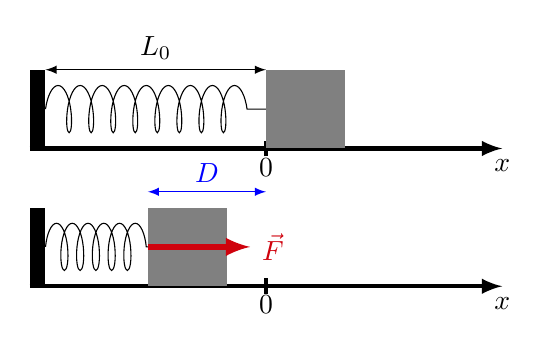
\begin{tikzpicture}[scale=1]
\tikzmath{
\L=2.;
\dx=0.75*\L;
\off=0.5;
\h=1;
}
\scalebox{1}{

\begin{scope}[shift={(0,1.75*\h)}]
\draw[-latex,line width=1.5pt] (-1.5*\L,0) -- (1.5*\L,0) node[below]{$x$};
\draw[line width=1.5pt] (0,-0.1) -- (0,0.1);
\node[below] at (0,0) {$0$};

\fill (-1.5*\L,0) rectangle (-1.4*\L,\h);
\draw[decoration={aspect=0.3, segment length=2.8mm, amplitude=3mm,coil},decorate] (-1.4*\L,\h/2) -- (0,\h/2);
\draw [latex-latex] (-1.4*\L,\h) -- (0,\h) node[midway,above]{$L_0$};
\fill[black!50] (0,0) rectangle (\h,\h);
\end{scope}
%%%%%%%%%%   compressed

\draw[-latex,line width=1.5pt] (-1.5*\L,0) -- (1.5*\L,0) node[below]{$x$};
\draw[line width=1.5pt] (0,-0.1) -- (0,0.1);
\node[below] at (0,0) {$0$};

\fill (-1.5*\L,0) rectangle (-1.4*\L,\h);
\draw[decoration={aspect=0.3, segment length=2mm, amplitude=3mm,coil},decorate] (-1.4*\L,\h/2) -- (-\dx,\h/2);
\draw [color=blue,latex-latex] (-\dx,1.2*\h) -- (0,1.2*\h) node[midway,above]{$D$};
\fill[black!50] (-\dx,0) rectangle (-\dx+\h,\h);
\draw[line width=2, -latex, color=myred] (-\dx,\h/2) -- +(1.3,0) node[right] {$\vec F$};

}
\end{tikzpicture}
\captionof*{figure}{\textit{Compressing a spring by a distance $D$.}}
\end{center}
}

%%%%%%%%%%%%%%%%%%%%%%%%%%%%%%%%
\twocolframe{Force varying with position (recap)}
{
\begin{itemize}
\item We can find the speed squared by applying the kinematic equation multiple times:
\begin{align*}
v_1^2&=v_0^2+2\frac{F_1}{m}\Delta x\\
v_n^2&=v_0^2+\frac{2}{m}\sum F_i\Delta x\\
\end{align*}
\item The velocity (squared) of the object as a function of position is given by:
\begin{align*}
v^2(x)=v_0^2+\frac{2}{m}\int F(x) dx
\end{align*}
\end{itemize}

}
{
\begin{center}
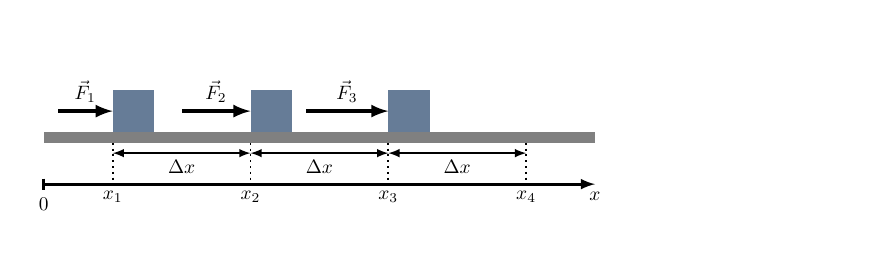
\begin{tikzpicture}[scale=1]
\tikzmath{
\L=10;
\h=0.75;
\w=0.2;
\dx=2.5;
\abox=0.75;
\Fm=1;
}
\scalebox{0.7}{
%axis
\draw[-latex, line width=1.5pt] (0,0) -- (\L,0) node[below]{$x$};
\draw[line width=1.5pt] (0,0.1) -- (0,-0.1) node[below]{$0$};
%floor
\fill[black!50] (0,\h) rectangle (\L,\h+\w);

\fill[color=myblue!60] (0.5*\dx,\h+\w) rectangle (0.5*\dx+\abox,\h+\w+\abox);
\fill[color=myblue!60] (1.5*\dx,\h+\w) rectangle (1.5*\dx+\abox,\h+\w+\abox);
\fill[color=myblue!60] (2.5*\dx,\h+\w) rectangle (2.5*\dx+\abox,\h+\w+\abox);

\draw[latex-,line width=2] (0.5*\dx,\h+\w+\abox/2) -- +(-\Fm,0) node[midway,above]{$\vec F_1$};
\draw[latex-,line width=2] (1.5*\dx,\h+\w+\abox/2) -- +(-1.25*\Fm,0) node[midway,above]{$\vec F_2$};
\draw[latex-,line width=2] (2.5*\dx,\h+\w+\abox/2) -- +(-1.5*\Fm,0) node[midway,above]{$\vec F_3$};

\draw[dotted, line width=1] (0.5*\dx,\h) -- +(0,-\h) node[below]{$x_1$};
\draw[dotted, line width=1] (1.5*\dx,\h) -- +(0,-\h) node[below]{$x_2$};
\draw[dotted, line width=1] (2.5*\dx,\h) -- +(0,-\h) node[below]{$x_3$};
\draw[dotted, line width=1] (3.5*\dx,\h) -- +(0,-\h) node[below]{$x_4$};

\draw[latex-latex, line width=1] (0.5*\dx,0.75*\h)--+(\dx,0) node[midway, below]{$\Delta x$};
\draw[latex-latex, line width=1] (1.5*\dx,0.75*\h)--+(\dx,0) node[midway, below]{$\Delta x$};
\draw[latex-latex, line width=1] (2.5*\dx,0.75*\h)--+(\dx,0) node[midway, below]{$\Delta x$};
}
\end{tikzpicture}
\captionof*{figure}{\textit{A block slides along $x$ with a force that changes depending on position}}
\end{center}
}


%%%%%%%%%%%%%%%%%%%%%%%%%%%%%%%%
\twocolframe{Force varying with position (recap)}
{
\begin{itemize}
\item A block is pushed against a spring, compressing it by a distance $D$. The force on the block (exerted by the spring) changes with position:
\begin{align*}
F(x)=-kx
\end{align*}
\item  Having released the block at rest ($v_0=0$) from $x = -D$, its speed when it reaches $x = 0$ is:
\begin{align*}
v^2(x=0)&=-\frac{2}{m}\int_{-D}^{0}kxdx=-\frac{2}{m}\left[\frac{1}{2}kx^2 \right]_{-D}^{0}\\
&=\frac{k}{m}D^2
\end{align*}
\end{itemize}

}
{
\begin{center}
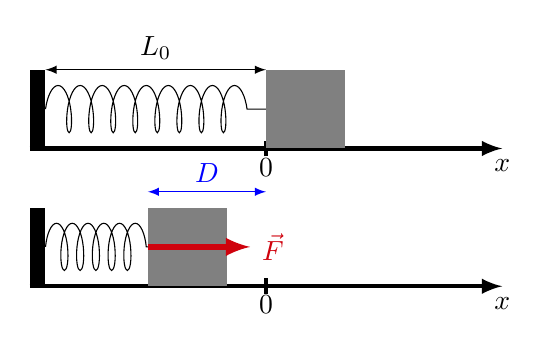
\begin{tikzpicture}[scale=1]
\tikzmath{
\L=2.;
\dx=0.75*\L;
\off=0.5;
\h=1;
}
\scalebox{1}{

\begin{scope}[shift={(0,1.75*\h)}]
\draw[-latex,line width=1.5pt] (-1.5*\L,0) -- (1.5*\L,0) node[below]{$x$};
\draw[line width=1.5pt] (0,-0.1) -- (0,0.1);
\node[below] at (0,0) {$0$};

\fill (-1.5*\L,0) rectangle (-1.4*\L,\h);
\draw[decoration={aspect=0.3, segment length=2.8mm, amplitude=3mm,coil},decorate] (-1.4*\L,\h/2) -- (0,\h/2);
\draw [latex-latex] (-1.4*\L,\h) -- (0,\h) node[midway,above]{$L_0$};
\fill[black!50] (0,0) rectangle (\h,\h);
\end{scope}
%%%%%%%%%%   compressed

\draw[-latex,line width=1.5pt] (-1.5*\L,0) -- (1.5*\L,0) node[below]{$x$};
\draw[line width=1.5pt] (0,-0.1) -- (0,0.1);
\node[below] at (0,0) {$0$};

\fill (-1.5*\L,0) rectangle (-1.4*\L,\h);
\draw[decoration={aspect=0.3, segment length=2mm, amplitude=3mm,coil},decorate] (-1.4*\L,\h/2) -- (-\dx,\h/2);
\draw [color=blue,latex-latex] (-\dx,1.2*\h) -- (0,1.2*\h) node[midway,above]{$D$};
\fill[black!50] (-\dx,0) rectangle (-\dx+\h,\h);
\draw[line width=2, -latex, color=myred] (-\dx,\h/2) -- +(1.3,0) node[right] {$\vec F$};

}
\end{tikzpicture}
\captionof*{figure}{\textit{Compressing a spring by a distance $D$.}}
\end{center}
}
%%%%%%%%%%%%%%%%%%%%%%%










%%%%%%%%%%%%%%%%%%%%%%%%%%

\section{Mathmatical Applications}
\label{sec:mathmaticalapplications}
\title{Mathmatical Applications}
\institute{Applying Newton's Laws}
\author{\insertsubsection}


%%%%%%%%%%%%%%%%%%%%%%%%%
\begin{frame}
\titlepage
\thispagestyle{empty}
\end{frame}

%%%%%%%%%%%%%%%%%%%%







%%%%%%%%%%%%%%%%%%%%%%%%%%%%%%%%
\subsection{Derrivation for force varying with position}
\begin{frame}{Mathematically, more formally}
\begin{itemize}
\item<1-> We know acceleration as a function of position:
\begin{align*}
\frac{dv}{dt}=a(x)=\frac{F(x)}{m}
\end{align*}
\item<2-> We cannot integrate over $t$, since $x$ (the position of where the force is applied) depends on $t$:
\begin{align*}
dv=a(x)dt
\end{align*}
\item<3-> We need to integrate over $x$, and change variables from $t$ to $x$:
\begin{align*}
\frac{dx}{dt}=v\rightarrow dt=\frac{1}{v}dx
\end{align*}
\item<4-> We can thus write
\begin{align*}
dv=a(x)dt=\frac{a(x)}{v}dx
\end{align*}
\end{itemize}
\end{frame}

%%%%%%%%%%%%%%%%%%%%%%%%%%%%%%%%
\begin{frame}{Mathematically, more formally}
\begin{itemize}
\item<1-> Think of the Chain Rule for the same result:
\begin{align*}
\frac{dv}{dx}&=\frac{dv}{dt}\frac{dt}{dx}=a\frac{1}{v}\\
\therefore dv &=\frac{a}{v}dx
\end{align*}
\item<2-> This allows us to ``separate variables'':
\begin{align*}
vdv=a(x)dx
\end{align*}
\item<3-> We can ``add together'' things on the right and the left, and they must still be equal:
\begin{align*}
\int_{v_0}^{v(x_1)}vdv&=\int_{x_0}^{x_1} a(x)dx\\
\frac{1}{2}v^2(x)-\frac{1}{2}v_0^2&=\int_{x_0}^{x_1} a(x)dx\\
\therefore v^2(x)&=v_0^2+2\int_{x_0}^{x_1} a(x)dx=v_0^2+\frac{2}{m}\int_{x_0}^{x_1} F(x)dx
\end{align*}
\end{itemize}
\end{frame}


%%%%%%%%%%%%%%%%%%%%%%%%%%%%%%%%
\begin{frame}{Mathematically, more formally}
\begin{itemize}
\item With constant acceleration, this just gives the kinematics equation:
\begin{align*}
v^2(x_1)&=v_0^2+2\int_{x_0}^{x_1} a(x)dx\\
&=v_0^2+2a(x_1-x_0)
\end{align*}
\item This is also where kinetic energy comes from (next week!)
\begin{align*}
v^2(x_1)&=v_0^2+\frac{2}{m}\int_{x_0}^x F(x)dx\\
\therefore \frac{1}{2}mv^2(x_1)-\frac{1}{2}mv_0^2&=\int_{x_0}^x F(x)dx
\end{align*}
Final kinetic energy minus initial kinetic energy is equal to Work done...
\end{itemize}
\end{frame}


%%%%%%%%%%%%%%%%%%%%%%%%%%%%%%%%
\subsection{Differential equations}
\label{subsec:differentialequations}
\begin{frame}{Differential equations}
\begin{itemize}
\item This is a differential equation:
\begin{align*}
vdv=a(x)dx
\end{align*}
\item We could write it as:
\begin{align*}
\frac{dv}{dx}=\frac{a(x)}{v}
\end{align*}
\item The derivative of a function $\frac{dv}{dx}$ depends on the function ($v(x)$) itself.
\item It is a \textbf{separable differential} equation, because we can separate all that depends on $v$ and $x$ onto separate sides of the equation (as in the first line). This allows us to find $v(x)$ by integrating both sides, as in the last slides.
\item Separable = usually easy to solve.
\item At this point, \textbf{you're not expected to solve a differential equation}, but you should understand the concept and how we're solving a separable equation. 
\end{itemize}

\end{frame}


%%%%%%%%%%%%%%%%%%%%%%%%%%%%%%%%
\subsection{Force varying with velocity}
\label{subsec:forcevaryingwithvelocity}
\twocolframest{Force varying with velocity (e.g. drag)}
{
\begin{itemize}
\item The force of drag (aka air resistance) depends on velocity.
\item Ultimately, it depends on the actual situation, sometimes it depends on $v$, sometimes on $v^2$.
\item The force also depends on the medium through which the object moves, and the size of the object.
\item Can model this as:
\begin{align*}
\vec F_d&=-b\vec v\\
\vec F_d&=-bv^2\hat v\\
\end{align*}
\end{itemize}
}
{
\begin{center}
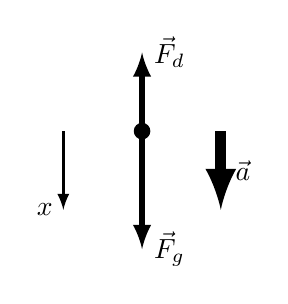
\begin{tikzpicture}[scale=1]
\tikzmath{
\L=2.;
\dx=0.75*\L;
\off=0.5;
\h=1;
}
\scalebox{1}{

\fill (0,0) circle (3pt);
\draw[-latex,line width=2] (0,0)--+(0,1.) node[right]{$\vec F_d$};
\draw[-latex,line width=2] (0,0)--+(0,-1.5) node[right]{$\vec F_g$};

\draw[-latex,line width=4] (1,0)--+(0,-1) node[midway,right]{$\vec a$};
\draw[-latex,line width=1] (-1,0)--+(0,-1) node[left]{$x$};
}
\end{tikzpicture}
\captionof*{figure}{\textit{A model for drag.}}
\end{center}
}


%%%%%%%%%%%%%%%%%%%%%%%%%%%%%%%%
\subsection{Example: linear drag force}
\twocolframe{Example: Drag linear with velocity}
{
\scriptsize
\begin{itemize}
\item We assume drag is linear (and write the $x$ component):
\begin{align*}
 F_d&=-b v\\
\end{align*}
\item<2-> Writing Newton's Second Law (which is a differential equation):
\begin{align*}
\sum F-x = mg-bv&=ma \\
mg-bv&= m\frac{dv}{dt}
\end{align*}
\item<3-> It's separable:
\begin{align*}
\frac{dv}{mg-bv}=-\frac{b}{m}dt
\end{align*}
\end{itemize}
}
{
\begin{center}
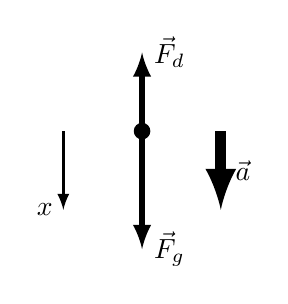
\begin{tikzpicture}[scale=1]
\tikzmath{
\L=2.;
\dx=0.75*\L;
\off=0.5;
\h=1;
}
\scalebox{1}{

\fill (0,0) circle (3pt);
\draw[-latex,line width=2] (0,0)--+(0,1.) node[right]{$\vec F_d$};
\draw[-latex,line width=2] (0,0)--+(0,-1.5) node[right]{$\vec F_g$};

\draw[-latex,line width=4] (1,0)--+(0,-1) node[midway,right]{$\vec a$};
\draw[-latex,line width=1] (-1,0)--+(0,-1) node[left]{$x$};
}
\end{tikzpicture}
\captionof*{figure}{\textit{A model for drag.}}
\end{center}
}


%%%%%%%%%%%%%%%%%%%%%%%%%%%%%%%%
\twocolframe{Example: Drag linear with velocity}
{
\begin{itemize}
\item<1-> So we can integrate both sides:
\begin{align*}
\int_0^{v(t_1)}\frac{dv}{mg-bv}dv=-\int_0^{t_1}\frac{b}{m}dt
\end{align*}
\item<2-> to find (after some math):
\begin{align*}
v(t_1)=\frac{mg}{b}\left(1-e^{-\frac{b}{m}t_1}\right)
\end{align*}
\end{itemize}
\only<2>{The speed increases asymptotically to the ``terminal velocity''. In the limit $t\to\infty$, we have:
\begin{align*}
v(t\to \infty) = \frac{mg}{b}
\end{align*}
}
}
{
\only<2>{
%\capfig{1}{figures/vterminal}{In the limit of $t\to\infty$, we have $v(t)=\frac{mg}{b}$, the object reaches ``terminal velocity''. This corresponds to the force of drag increasing until it reaches the magnitude of the force of gravity.}
\vspace{-1.5cm}
\begin{center}
 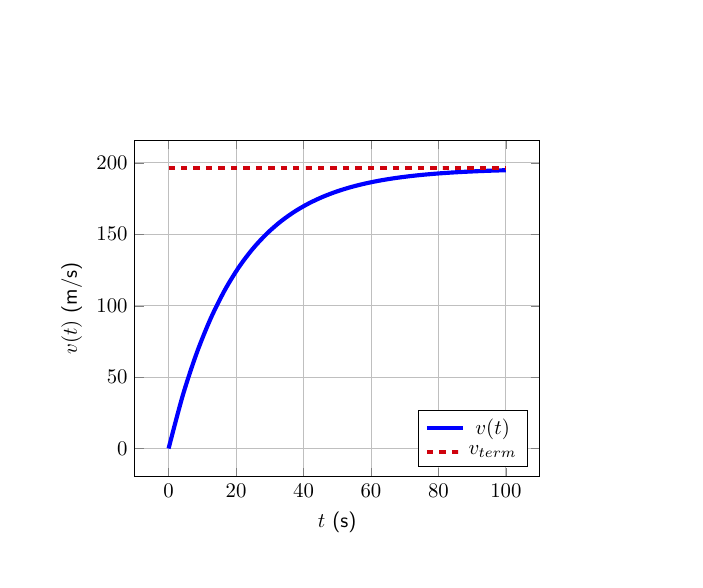
\begin{tikzpicture}
 \tikzmath{
 \ma=10;
 \b=0.5;
 }
 \scalebox{0.75}{
 \begin{axis}[domain = 0:100, grid,legend pos=south east,xlabel=$t$ (s), ylabel=$v(t)$ (m/s)]
  \addplot[smooth,color=blue,line width=2] {(\ma*9.81/\b)*(1-exp(-\b/\ma*x)};
  \addplot[smooth,dashed,color=myred,line width=2] {\ma*9.81/\b};

  \addlegendentry{$v(t)$}
  \addlegendentry{$v_{term}$}


 \end{axis}

 }
 \end{tikzpicture}
 \captionof*{figure}{\textit{Speed as a function of time for an object that started from rest and falls with drag. The object has a mass of $m=\SI{10}{kg}$ and the coefficient of drag is given by $b=\SI{0.5}{N\cdot s/m}$}.}
\end{center}


}
\only<1>{

\begin{center}
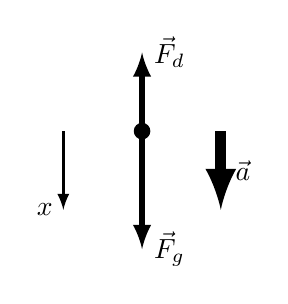
\begin{tikzpicture}[scale=1]
\tikzmath{
\L=2.;
\dx=0.75*\L;
\off=0.5;
\h=1;
}
\scalebox{1}{

\fill (0,0) circle (3pt);
\draw[-latex,line width=2] (0,0)--+(0,1.) node[right]{$\vec F_d$};
\draw[-latex,line width=2] (0,0)--+(0,-1.5) node[right]{$\vec F_g$};

\draw[-latex,line width=4] (1,0)--+(0,-1) node[midway,right]{$\vec a$};
\draw[-latex,line width=1] (-1,0)--+(0,-1) node[left]{$x$};
}
\end{tikzpicture}
\captionof*{figure}{\textit{A model for drag.}}
\end{center}
}
}






%%%%%%%%%%%%%%%%%%%%%%%%%%%%%%%%

\section{Building Models}
\label{sec:buildingmodels}
\title{Building Models Using Newton's Laws}
\institute{Applying Newton's Laws}
\author{\insertsubsection}


%%%%%%%%%%%%%%%%%%%%%%%%%
\begin{frame}
\titlepage
\thispagestyle{empty}
\end{frame}


%%%%%%%%%%%%%%%%%%%%%%%%%%%%%%%%











%%%%%%%%%%%%%%%%%%%%%%%%%%%%%%%%
\subsection{Applying Newton's Laws}
\label{subsec:applyingnewtonslaws}
\twocolframesf{Reminder: Applying Newton's Laws}
{\scriptsize
Strongly recommend the following procedure for model building:
\begin{enumerate}
\item \textbf{Make a very good Free Body Diagram} for each mass that shows:
\begin{enumerate}
\scriptsize
\item All the forces (``what could be pushing or pulling on the mass?'').
\item The acceleration vector.
\item Relevant angles.
\item Your choice of coordinate system (make $+x$ parallel to acceleration).
\end{enumerate}
\item Read off the free-body diagram(s) to write Newton's Second Law, you get one equation per dimension:
\begin{align*}
\sum F_x = ma \quad \sum F_y=0
\end{align*}
 (if you chose x-axis parallel to acceleration, not always possible).
\item You now have a series of equations, just do some math to solve for any variables you need.
\end{enumerate}

}
{
\vspace{-1cm}
\begin{center}
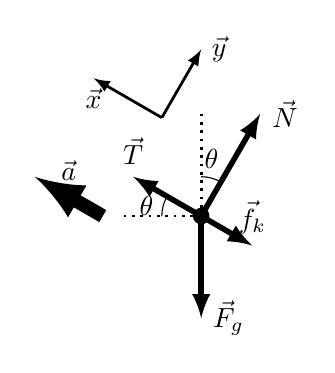
\begin{tikzpicture}[scale=1]
\tikzmath{
\th=30;
\no=1.5;
\vg=cos(\th)*\no;
\fk=0.75;
}
\pgfmathsetmacro{\T}{1}
\scalebox{1}{
\coordinate (P) at (0,0);

\fill (P) circle(3pt);
\draw[-latex, line width=2] (P) -- (0,-\vg) node[right]{$\vec F_g$};
\draw[-latex, line width=2] (P) -- (90-\th:\no) node[right]{$\vec N$};
\draw[-latex, line width=2] (P) -- (180-\th:\T) node[above]{$\vec T$};
\draw[-latex, line width=2] (P) -- (-\th:\fk) node[above]{$\vec f_k$};

\draw[dotted, line width=1] (P) -- +(0,\vg);
\draw ($(P)+(0,0.5)$) arc(90:90-\th:0.5) node[midway,above]{$\theta$};

\draw[dotted, line width=1] (P) -- +(-\T,0);
\draw ($(P)+(-0.5,0)$) arc(180:180-\th:0.5) node[midway,left]{$\theta$};


\draw[-latex, line width=1] ($(P)+(-0.5,1.25)$) -- +(180-\th:1) node[below]{$\vec x$};
\draw[-latex, line width=1] ($(P)+(-0.5,1.25)$) -- +(90-\th:1) node[right]{$\vec y$};
\draw[-latex, line width=5] ($(P)+(-1.25,0)$) -- +(180-\th:1) node[midway,above]{$\vec a$};

}
\end{tikzpicture}
\captionof*{figure}{\textit{Reading off your very good free body diagram}}
\end{center}
\scriptsize
Reading off the diagram to write Newton's Second Law:
\begin{align*}
\sum F_x&: &T-f_k-F_g\sin\theta &= ma \\
\sum F_y&: &N-F_g\cos\theta &=0
\end{align*}
}


%%%%%%%%%%%%%%%%%%%%%%%%%%%%%%%%
\subsection{Circular motion with Newton's laws}
\label{subsec:circularmotionwithnewtonslaws}
\label{subsec:}
\begin{frame}{Newton’s Laws and Circular motion}
\begin{itemize}
\item In circular motion (motion along a circle):
\begin{itemize}
\item The velocity is always tangent to the circle.
\item \textbf{There is always a centripetal component of acceleration} (radial acceleration, perpendicular to the velocity, responsible for changing the direction of $\vec v$).
\item There can be a tangential component of the acceleration, if the object changes speed (\textbf{non-uniform} circular motion).
\item The angular quantities ($\theta,\omega,\alpha$) are related to the tangential quantities (e.g. $v=\omega R$, $a_T=\alpha R$ ).
\end{itemize}
\item The sum of the forces must be parallel to the total acceleration:
\begin{align*}
\sum \vec F=m\vec a
\end{align*}
\item Can break this up into radial and tangential components (a good choice of $xy$):
\begin{align*}
\sum F_R&=ma_R=m\frac{v^2}{R}=m\omega^2R\quad \text{(Radial component, never zero)}\\
\sum F_T&=ma_T=m\alpha R\quad \text{(Tangential component, zero if uniform circ. mot.)}
\end{align*}
\end{itemize}
\end{frame}



%%%%%%%%%%%%%%%%%%%%%%%%%%%%%%%%
\subsection{Two masses on accelerating turntable}
\label{subsec:twomassesonacceleratingturntable}
\twocolframesf{Two masses on accelerating turntable}
{\scriptsize
\begin{itemize}
\item Both tangential and radial acceleration, only force of static friction can result in acceleration.
\item Both masses have the same angular velocity ($\omega$) and angular acceleration ($\alpha$).
\item Masses stay while $f_s\leq \mu_sN=\mu_smg$.
\item Tangential (linear) acceleration (constant):
\begin{align*}
ma_T=m\alpha r=f_{sT}
\end{align*}
\item Radial (linear) acceleration (increasing):
\begin{align*}
ma_R=m\omega^2r=f_{sR}
\end{align*}
\item Magnitude of the force of friction:
\begin{align*}
f_s=\sqrt{f_{sT}^2+f_{sR}^2}=mr\sqrt{\alpha^2+\omega^2}\leq mg\\
\therefore r\sqrt{\alpha^2+\omega^2}\leq g
\end{align*}
\end{itemize}
}
{
\begin{center}
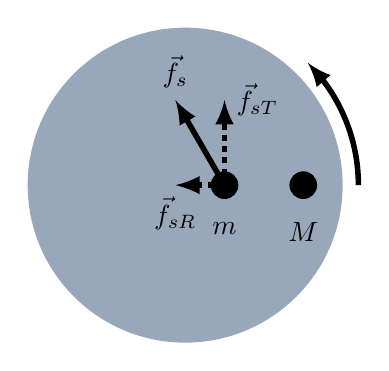
\begin{tikzpicture}[scale=1]
\tikzmath{
\R=2;
\th=30;
\fss=1.25;
\fst=\fss*cos(\th);
\fsr=-\fss*sin(\th);
}
\scalebox{1}{
\coordinate (C) at (0,0);

\fill[myblue!40] (C) circle(\R);
\fill[] ($(C)+(0.25*\R,0)$) circle(5pt);
\fill[] ($(C)+(0.75*\R,0)$) circle(5pt);
\node[below=10pt] at ($(C)+(0.25*\R,0)$) {$m$};
\node[below=10pt] at ($(C)+(0.75*\R,0)$) {$M$};

\draw[-latex, line width=2] ($(C)+(0.25*\R,0)$) --+(\fsr,\fst) node[above]{$\vec f_s$};
\draw[-latex,dotted, line width=2] ($(C)+(0.25*\R,0)$) --+(\fsr,0) node[below]{$\vec f_{sR}$};
\draw[-latex,dotted, line width=2] ($(C)+(0.25*\R,0)$) --+(0,\fst) node[right]{$\vec f_{sT}$};

\draw[-latex, line width=2] (1.1*\R,0) arc (0:45:1.1*\R);
}
\end{tikzpicture}
\captionof*{figure}{\textit{Two masses on an accelerating turntable.}}
\end{center}
\only<2>{
\textcolor{myred}{Since $\alpha$ and $\omega$ are the same for both masses, the one with the larger value of $r$ will fall of first, regardless of mass!}
}
}

%%%%%%%%%%%%%%%%%%%%%%%%%%%%%%%%


%%%%%%%%%%%%%%%%%%%%%%%%%%%%%%%%
\subsection{Uniform circular motion}
\label{subsec:uniformcircularmotion}
\twocolframesf{Modeling \textit{uniform} circular motion}
{
\begin{itemize}
\item Uniform means constant speed (no tangential acceleration).
\item The \textbf{net acceleration} is towards the centre of the circle:
\begin{align*}
a_C=a_R=m\frac{v^2}{R}
\end{align*}
\item The \textbf{sum of the forces} is directed towards the centre of the circle:
\begin{align*}
\sum F_R&=m\frac{v^2}{R}\\
\sum F_T&=0\\
\end{align*}
\end{itemize}
}
{

 \begin{tikzpicture}[scale=1]
 \scalebox{1}{
  \coordinate (P1) at (-3,0);
  \node at (0,0) {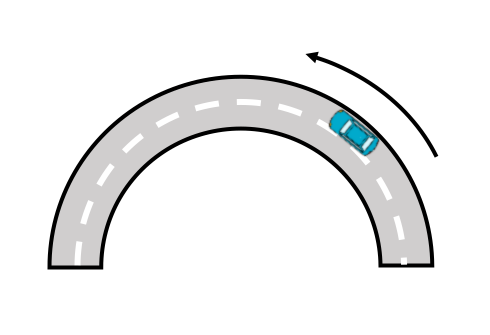
\includegraphics[scale=0.3]{figures/ApplyingNewtonsLaws/car2.png}};
  \fill[] (0,-1) circle(2pt);
  \draw[dotted,line width=1](0,-1) -- +(50:1.8)node[midway,below]{$R$}; 
 }
\end{tikzpicture}
\captionof*{figure}{\textit{Top view of car going around a corner}}
}


%%%%%%%%%%%%%%%%%%%%%%%%%%%%%%%%

%%%%%%%%%%%%%%%%%%%%%%%%%%%%%%%%
\subsection{Banked curves}
\label{subsec:bankedcurves}
\begin{frame}{Banked curves}
\begin{itemize}
\item By banking the road, one can change the direction of the normal force so that it, too, can have a component towards the centre of the circle
\end{itemize}
\begin{columns}[]

 \column{0.5\textwidth}
 \vspace{0.7cm}
 \begin{tikzpicture}[scale=1]
 \scalebox{1}{
  \coordinate (P1) at (-3,0);
  \node at (0,0) {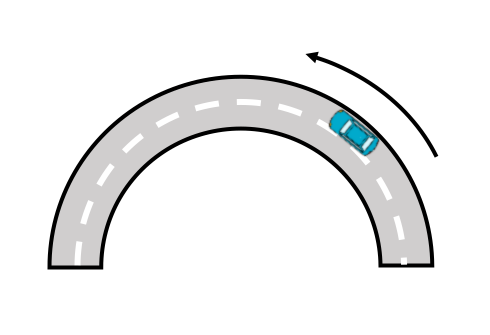
\includegraphics[scale=0.3]{figures/ApplyingNewtonsLaws/car2.png}};
  \fill[] (0,-1) circle(2pt);
  \draw[dotted,line width=1](0,-1) -- +(50:1.8)node[midway,below]{$R$}; 
 }
\end{tikzpicture}
\captionof*{figure}{\textit{Top view of car going around a corner}}
 
\column{0.5\textwidth}
 
\begin{tikzpicture}[scale=1]
\tikzmath{
\L=4;
\h=1.3;
\no=1.75;
\th=atan(\h/\L);
\nox=\no*sin(\th);
\noy=\no*cos(\th);
}
 \scalebox{1}{
  \coordinate (P1) at (1.75,1.15);
  \coordinate (P2) at ($(P1)+(0,1.5)$);
  
  \draw[line width=2] (\L,\h) -- (\L,0) -- (0,0) --cycle;
  
  \node at (P1) {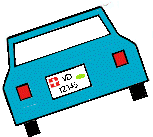
\includegraphics[scale=0.3]{figures/ApplyingNewtonsLaws/tiltedcar.png}};
  \draw (1,0) arc (0:\th:1) node[midway,right]{$\theta$};
  
  \draw[line width=1.5, dotted] (-1.5,1.15) -- (1.6, 1.15) node[midway,above]{$R$};
  
  \fill (P2) circle(3pt);
  \draw[line width=2,-latex] (P2) -- +(90+\th:\no) node[right]{$\vec N$};
  \draw[line width=1.5,-latex,color=myred] (P2) -- +(-\nox,0) node[midway,below] {$N\sin\theta$};
  \draw[dotted, line width=1] ($(P2)+(-\nox,0)$) -- +(0,\noy) node[midway,right=-3pt] {$\theta$};
 }
\end{tikzpicture}
\captionof*{figure}{\textit{Side view of car going around a banked curve.}}
 
\end{columns}
\end{frame}


%%%%%%%%%%%%%%%%%%%%%%%%%%%%%%%%


%%%%%%%%%%%%%%%%%%%%%%%%%%%%%%%%


%%%%%%%%%%%%%%%%%%%%%%%%%%%%%%%%
\subsection{Vertical Circle}
\label{subsec:verticalcircle}
\twocolframesf{Motion in a vertical circle}
{\begin{itemize}
\item What you did as an experiment in RA5.
\item A ball swinging around a rope, with a force of tension.
\item A roller coaster, with a normal force instead of tension. 
\end{itemize}
\textit{It can never be uniform circular motion, there will always be a tangential component to acceleration from gravity (except at the top and bottom).}
}
{
\begin{center}
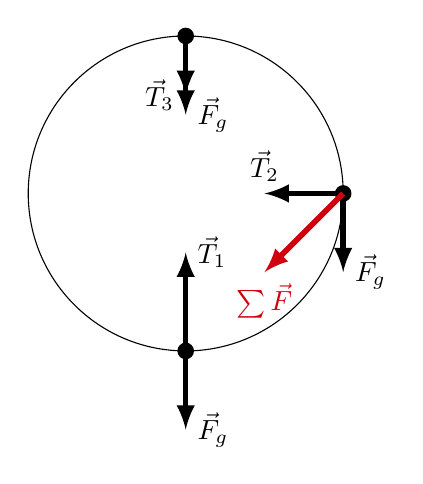
\begin{tikzpicture}[scale=1]
\tikzmath{
\R=2;
\vg=1;
\t=1.25*\vg;
\tt=\vg;
\ttt=0.75*\vg;
}
\scalebox{1}{
\coordinate (C) at (0,0);
\coordinate (P1) at (0,-\R);
\coordinate (P2) at (\R,0);
\coordinate (P3) at (0,\R);


\draw (C) circle(\R);

\fill (P1) circle(3pt);
\fill (P2) circle(3pt);
\fill (P3) circle(3pt);

\draw[-latex, line width=2] (P1) -- +(0,-\vg) node[right]{$\vec F_g$};
\draw[-latex, line width=2] (P1) -- +(0,\t) node[right]{$\vec T_1$};

\draw[-latex, line width=2] (P2) -- +(0,-\vg) node[right]{$\vec F_g$};
\draw[-latex, line width=2] (P2) -- +(-\tt,0) node[above]{$\vec T_2$};
\draw[-latex, line width=2,color=myred] (P2) -- +(-\tt,-\vg) node[below]{$\sum \vec F$};

\draw[-latex, line width=2] (P3) -- +(0,-\vg) node[right]{$\vec F_g$};
\draw[-latex, line width=2] (P3) -- +(0,-\ttt) node[left]{$\vec T_3$};
}
\end{tikzpicture}
\captionof*{figure}{\textit{A mass on a string going around in a vertical circle. The sum of the forces only points to the centre of the circle at the top and bottom.}}
\end{center}
}


%%%%%%%%%%%%%%%%%%%%%%%%%%%%%%%%


%%%%%%%%%%%%%%%%%%%%%%%%%%%%%%%%



%%%%%%%%%%%%%%%%%%%%%%%%%%%%%%%%



%%%%%%%%%%%%%%%%%%%%%%%%%%%%%%%%



%%%%%%%%%%%%%%%%%%%%%%%%%%%%%%%%



%%%%%%%%%%%%%%%%%%%%%%%%%%%%%%%%



%%%%%%%%%%%%%%%%%%%%%%%%%%%%%%%%



%%%%%%%%%%%%%%%%%%%%%%%%%%%%%%%%



%%%%%%%%%%%%%%%%%%%%%%%%%%%%%%%%



%%%%%%%%%%%%%%%%%%%%%%%%%%%%%%%%



%%%%%%%%%%%%%%%%%%%%%%%%%%%%%%%%



%%%%%%%%%%%%%%%%%%%%%%%%%%%%%%%%



%%%%%%%%%%%%%%%%%%%%%%%%%%%%%%%%



%%%%%%%%%%%%%%%%%%%%%%%%%%%%%%%%






\end{document}